\chapter{Approach 1: Signal Mapping}

The first approach we will develop is an idea called \textbf{Signal Mapping}. Accounts have attributes, and when we look at the accounts for two subsequent years, we can observe changes in these attributes. We will see that from these changes, we can derive signals, which can be mapped to appropriate musical constructs. These constructs can be arranged together to form music. To do this, we will be working with the account \textbf{balance sheet}.


\section{Notation and Definitions}

\begin{center}
\begin{singlespace}
\begin{tabular}{ l l }
\hline
\hline
\textbf{\{ $\ldots$ \}} & A set of items \\ \hline
\textbf{Sequence} & An ordered set which can contain repeating elements \\ \hline
\textbf{List} & Another name for a Sequence \\ \hline
\textbf{$\langle \ldots \rangle$} & A sequence of items \\ \hline
\textbf{Musical sequence}: & A finite sequence of notes. \\ \hline
\textbf{Set of musical sequences}: & Multiple musical sequences whose feel is governed by the set of \\
 & musical attributes. \\ \hline
\textbf{Musical attribute}: & A static value which pre-determines the feel of a musical sequence. \\
 & For example: tempo, time signature or key signature. \\ \hline
\textbf{Set of musical attributes}: & Multiple non-contradicting musical attributes. \\ \hline
\textbf{Musical movement}: & The set of musical sequences as governed by the set of musical \\
& attributes \textit{(i.e. the complete music generated by the accounts)}. \\ \hline
\hline
\end{tabular}
\end{singlespace}
\end{center}



\section{Problem Discussion}

Recall that an account's balance sheet consists of five attributes. Recall also that to assess the health of a company, we can compare the balance sheets between two subsequent years.

Now consider the diagram given in \textit{figure \ref{fig:ss01}}. We can connect two parameters together to produce a unique \textbf{signal}. This signal can then be routed to a \textbf{processor}, which converts it into a musical sequence. Continuing onwards by piping the output signals of multiple processors produces a complete movement of music. By tweaking and fine tuning the settings of these processors, we can harness the sound so that it represents the account's data.



\begin{figure}[ht]
\centering
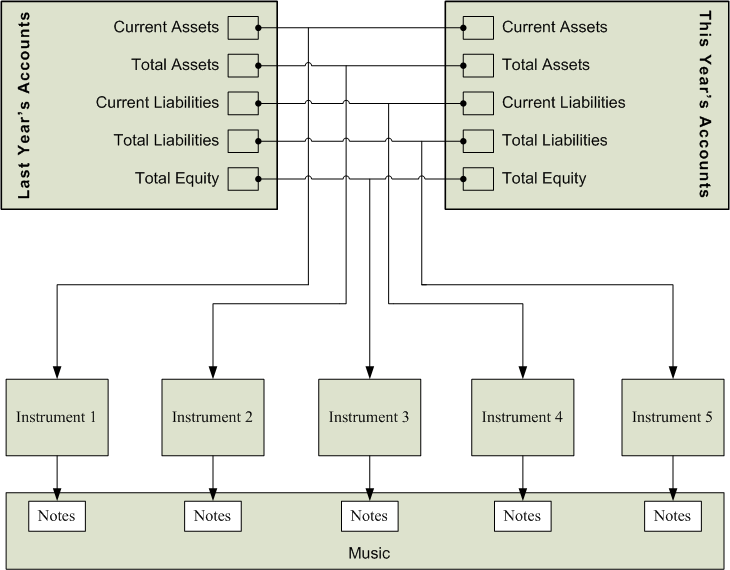
\includegraphics[scale=0.5]{ss01}
\caption{Mapping of account information to music. Each item of the account is independently mapped to a musical sequence.}
\label{fig:ss01}
\end{figure}

\noindent Essentially, we are mapping the difference between two parameters to a musical sequence or musical attribute. The processors are `black boxes', and the overall picture is only concerned with the signals going in and out of the processors. In other words, each processor will correspond to a function in the program.

Looking inside one of these processors, there would be an algorithm to take the account values and turn them into a suitable musical sequence. The processors will have `dials' which when modified change variables within the algorithm. It is these settings that we will tweak to fine tune the system, so that it produces the musical output we are looking for.



\section{Processor Isolation: A Sequential Approach}

The most crucial issue we are concerned with is that the overall sound produced must reflect the overall state of the accounts.  Although we are mapping individual account details to individual musical elements, we have to ensure that the overall �feel� of the sound fits the overall state of the accounts. 

The first approach we will try is to have each signal routed to an isolated processor. This processor generates a musical sequence. These sequences are played sequentially, one after the other. The result is a musical sequence in the form of a melody, which gives an impression of the account.

As some changes are more significant than other changes (bigger change in values of account attribute between years), we order the signals in terms of \textbf{magnitude}. This way, the individual musical sequences are joined up in order of importance.

We also need a way of deriving musical attributes which affect the \textit{whole} musical sequence. To do this, we calculate a \textbf{compound signal} which represents the overall signal spread.


\begin{figure}[ht]
\centering
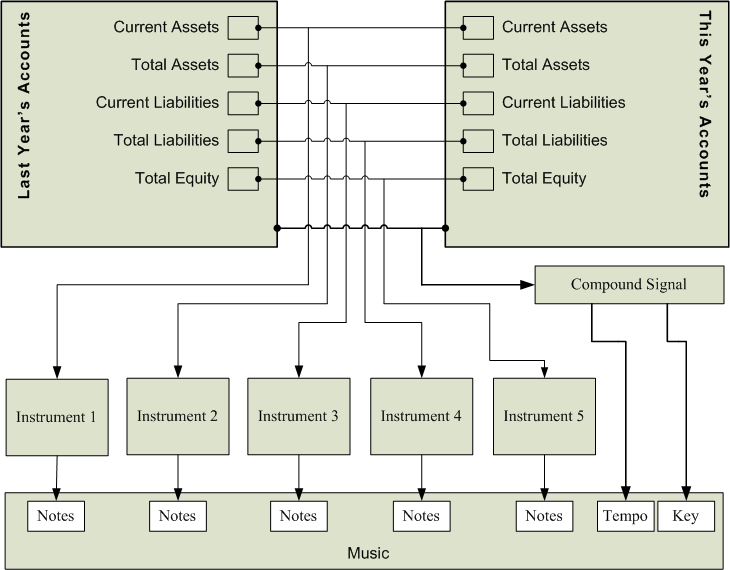
\includegraphics[scale=0.5]{ss02}
\caption{Mapping with a compound signal to control tempo and key. The compound signal is derived from the set of individual signals.}
\label{fig:ss02}
\end{figure}

\noindent 



\section{Processor Interaction: A Parallel Approach}

With the ability to play several musical sequences in sequence, we can modify this approach to produce music where the sequences play concurrently \textit{(figure \ref{fig:ss03})}. Taking this approach has the advantage of creating a completely different sound to the sequential approach, which we can compare with later.

\begin{figure}[ht]
\centering
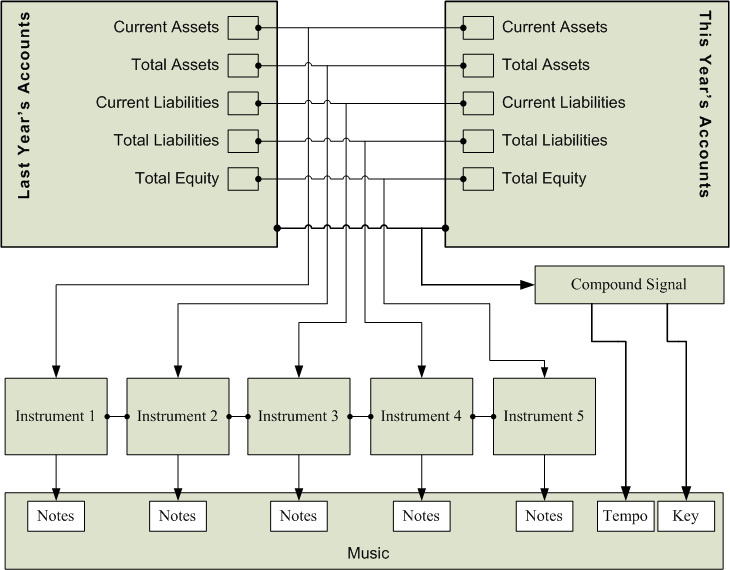
\includegraphics[scale=0.5]{ss03}
\caption{Mapping with sequences in parallel.}
\label{fig:ss03}
\end{figure}

\noindent However doing this presents us with a new problem. As each of the note sequences generated by the processors are in their own key, if we attempt to play them together, there will note clashes and general discordance of notes. Seeing as we are aiming to generate \textit{music}, this situation is clearly undesirable, and so we need a strategy to account for this. As an example, let's take the following two arbitrary note sequences:

\begin{singlespace}
\begin{formality}
$Seq_{1} = \langle C\#, F, A\# \rangle $ \\
$Seq_{2} = \langle E\#, F\#, C \rangle $
\end{formality}
\end{singlespace}

Some of these notes will clash if the sequences are played in parallel (for example, the 2nd item in each list). Additionally, if we are to adhere to a proper musical structure, we need an overall key to which all sequences should reside in.

To solve this problem, we invent the concept of a \textbf{keymap}. A keymap is a list of allowed notes, and will usually specify a scale of notes in the overall key. For example, consider the scale of C major:

\begin{singlespace}
\begin{formality}
$KeyMap = \langle C, D, E, F, G, A, B \rangle$
\end{formality}
\end{singlespace}

\noindent We map the notes of $Seq_{1}$ and $Seq_{2}$ to the notes in $KeyMap$ via the following algorithm:

\begin{singlespace}
\begin{formality}
\begin{itemize}
\item[\textbullet] \texttt{For each Note in Seq:}
	\begin{itemize}
	\item[\textbullet] \texttt{If Note not in KeyMap then:}
		\begin{itemize}
		\item[\textbullet] \texttt{If Note - 1 in KeyMap then:}
			\begin{itemize}
			\item[\textbullet] \texttt{Note = Note - 1}
			\end{itemize}
		\end{itemize}
		\item[\textbullet] \texttt{else:}
			\begin{itemize}
			\item[\textbullet] \texttt{Repeat until Note in KeyMap:}
				\begin{itemize}
				\item[\textbullet] \texttt{Note = Note + 1}
				\end{itemize}
			\end{itemize}
	\end{itemize}
\end{itemize}
\end{formality}
\end{singlespace}

\noindent Running the algorithm would re-map $Seq_{1}$ and $Seq_{2}$ as follows:

\begin{singlespace}
\begin{formality}
$Seq_{1} = \langle C, F, A \rangle $ \\
$Seq_{2} = \langle E, F, C \rangle $
\end{formality}
\end{singlespace}

\section{From Signals to Music}

So far, we have looked at the overall picture; individual elements of an account are mapped to individual elements of music. The next step is to discuss the activity within the processors, so that an individual account attribute is mapped to a \textit{representative musical element}. \\

Each processor will receive two values; one from the same attribute in each of the two account sheets. The output musical sequence could be attributed to a member of a set of pre-set sequences. This musical sequence can then be `stretched' or `squashed' according to the spread of the values from the accounts, and its starting note may also be set independently of the default. For mapping account data to musical attributes, output may be as simple as a single value (such as a tempo). For example, let \textit{S} be the set of types of musical sequences given by:

\begin{singlespace}
\begin{formality}
$S \rightarrow \{scale\_ascend, scale\_descend, broken\_chord\_ascend, \\broken\_chord\_descend, arpeggio\_ascend, arpeggio\_descend\}$
\end{formality}
\end{singlespace}

\noindent Each of these musical sequences has an attribute associated with it, which will determine how far the spread is between the start and end note. The sound of the sequence will depend on the musical attribute generated for the final movement (a minor key signature will mean that \textit{scale\_ascend} will be in a minor key, as will all members of \textit{S}).

If we take an arbitrary account, we may end up with a musical output as described below.

Let $M$ be the full musical movement (consisting of the set of musical sequences and the set of musical attributes):

\begin{singlespace}
\begin{formality}
$M \rightarrow \{I, A\}$
\end{formality}
\end{singlespace}

\noindent Let us take a set $I$ to be the set of musical sequences for four fields in the account sheet:

\begin{singlespace}
\begin{formality}
$I \rightarrow \{I_{1}, I_{2}, I_{3}, I_{4}\}$
\end{formality}
\end{singlespace}

\noindent Let $start$ (the starting note) and $spread$ (the amount of stretching) be attributes of $I$. Let the members of \textit{I} in our arbitrary example be defined as follows:

\begin{singlespace}
\begin{formality}
$I_{1} = scale\_ascend (root = A, tonic = major)$ \\
$I_{2} = scale\_ascend (root = C, tonic = major)$ \\
$I_{3} = arpeggio\_descend (root = A, tonic = minor)$ \\
$I_{4} = broken\_chord\_descend (root = F, tonic = minor)$
\end{formality}
\end{singlespace}

\noindent Let $A$ be the set of musical attributes for $M$:

\begin{singlespace}
\begin{formality}
$A \rightarrow \{A_{tempo}, A_{key\_signature}\}$
\end{formality}
\end{singlespace}

\noindent Let the members of $A$ be defined as follows:

\begin{singlespace}
\begin{formality}
$A_{tempo} = 100bpm \\
A_{key\_signature} = B minor$
\end{formality}
\end{singlespace}

\noindent The above representation would define a musical movement consisting of four instruments. Two of these instruments are playing ascending scales (beginning at A and C respectively, and the second jumping two tones each beat of the bar). The third will play a descending arpeggio beginning on A, and the fourth will play a descending scale beginning with F. As the key signature is defined as B minor, the notes of the scales and arpeggios will correspond to the notes in this scale. The speed this movement will be played at is 100 beats per minute.



\section{Signal Generation}

At this stage, we must step back and consider the important issue of signal generation. How exactly can we generate a signal from account attributes? To do this, we first need to define what a signal is, in the context of Financial Music.

\begin{singlespace}
\begin{formality}
\textbf{Definition:} A signal generated for an account attribute is a \textbf{ratio} of the attributes between two years with respect to direction of change.
\end{formality}
\end{singlespace}

\noindent It is easier to understand what is meant by the above definition through the use of an example. Consider the following account:

\small
\begin{center}
\begin{singlespace}
\begin{tabular}{ | l || l | l | l | l | l | }
\hline
 & \textbf{Current Assets} & \textbf{Total Assets} & \textbf{Current Liabilities} & \textbf{Total Liabilities} & \textbf{Total Equity} \\ \hline \hline
Year 1 & 4546723 & 11716362 & 3551852 & 8345658 & 3370704 \\ \hline
Year 2 & 3769524 & 10607753 & 3200228 & 7403901 & 3203852 \\
\hline
\end{tabular}
\end{singlespace}
\end{center}
\normalsize

\noindent A ratio for an account attribute $i$ is derived as follows:

\begin{singlespace}
\begin{formality}
$S = $\LARGE$\frac{year1_{i}}{year2_{i}}$\normalsize
\end{formality}
\end{singlespace}

\noindent In the case of the example account, we would generate a list of ratios, which would appear as the following list:

\begin{singlespace}
\begin{formality}
$\langle 1.2061796131288725, 1.1045093150264718, 1.1098746714296606, 1.1271974057999965,\\1.0520785604328788 \rangle$
\end{formality}
\end{singlespace}

\noindent The signals can be interpreted as follows:

\begin{singlespace}
\begin{formality}
$S \textless 1 \Rightarrow decreasing$ \\
$S \textgreater 1 \Rightarrow increasing$ \\
$S = 1 \Rightarrow unchanged$
\end{formality}
\end{singlespace}

\noindent At this point, there is a serious issue that needs to be addressed. In forming the ratio by dividing the account attribute from the first year by the same attribute from the second year, we have made the assumption that an increase between years is always desirable.

This is not always the case, and we need to look at which attributes this applies to. For these attributes, an increase in liabilities over the course of a year is considered bad, and we should adjust the ratios of \textit{current liabilities} and \textit{total liabilities} to reflect this. This can be done by defining a list as follows:

\begin{singlespace}
\begin{formality}
$R = \langle false, false, true, true, true\rangle$
\end{formality}
\end{singlespace}

\noindent If we using this list as we are generate the ratios, if the attribute's position in $R$ is $true$, then we reverse the ratio such that for attribute $i$:

\begin{singlespace}
\begin{formality}
$R_{i} = false \Rightarrow S_{i} = $\LARGE$\frac{year1_{i}}{year2_{i}}$\normalsize, \hspace{20pt}$ R_{i} = true \Rightarrow S_{i} = $\LARGE$\frac{year2_{i}}{year1_{i}}$\normalsize
\end{formality}
\end{singlespace}

\noindent Doing this now results in a correct list of ratios (the altered values are underlined):

\begin{singlespace}
\begin{formality}
$\langle 1.2061796131288725, 1.1045093150264718, \underline{0.90100263186641782}, \underline{0.88715605168579881},\\1.0520785604328788 \rangle$
\end{formality}
\end{singlespace}

\noindent These ratios are the representation of our \textbf{signals}, and will be referred to by the term `signals' from this point onwards.



\section{Generating a Compound Signal}

In order to set a tempo and initial key, we need to generate a signal which represents the overall state of the account. This is the compound signal, and is generated by taking an average of the five signals generated from the account attributes. With a set of signals at our disposal, we can now map these to musical sequences.


\section{Mapping Signals to Music}

In this Signal Mapping approach, we have formulated the idea of `processors' which turn a signal into a music sequence. But, how is this done?

In professional music sequencing software, a series of effects may be added to each channel to process the sound before it's heard. These effect boxes process the sound as it travels through. These processors are in effect empty boxes which can be `skinned' with a chosen algorithm. The algorithmic skins are stored as entities separate to the processor (figure: \ref{fig:map04}).

\begin{figure}[ht]
\centering
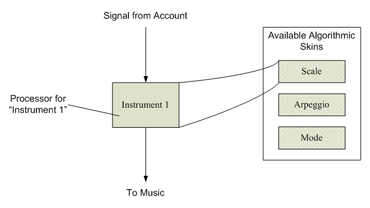
\includegraphics[scale=0.75]{Mapping_04}
\caption{Showing how a processor can be skinned from a selection of choices.}
\label{fig:map04}
\end{figure}

\noindent The skins themselves have a number of field values which can be set to make the processor's sound differ from other processors with the same skin (figure: \ref{fig:map05}).

\begin{figure}[ht]
\centering
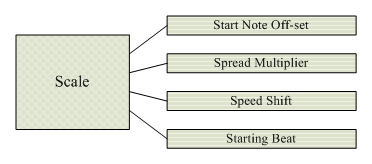
\includegraphics[scale=0.75]{Mapping_05}
\caption{Attributes of a scale, which can be set to values in order to produce a unique sound.}
\label{fig:map05}
\end{figure}

\noindent This modular approach allows for each processor to choose its skin based on the nature of the input signal. For simplicity�s sake, we will allow each processor to have only one skin applied to it. The processors work by having the signals `trigger' musical sequences by passing \textbf{threshold levels}. To understand this concept, consider the following proposition for a signal $S$ which produces musical sequence $M$:

\begin{singlespace}
\begin{formality}
$S \in \mathbbm{R}^{+}$ \\
$S \textless 0.15 \Rightarrow M = Scale$ \\
$S \textless 0.3 \Rightarrow M = Arpeggio$ \\
$S \geq 0.3 \Rightarrow M = Broken Chord$
\end{formality}
\end{singlespace}

\noindent Therefore, if we have an input signal strength of 0.14, we get a scale returned, as this signal strength is below the threshold for a scale \textit{(figure \ref{fig:sigmet01})}.

\begin{figure}[ht]
\centering
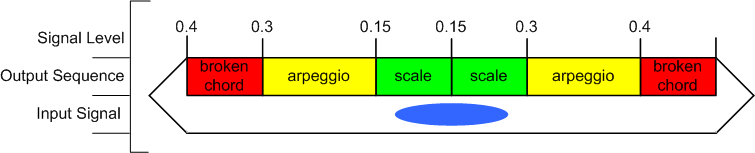
\includegraphics[scale=0.5]{sigmet01}
\caption{Diagram showing how an input signal will result in an output musical sequence by passing a threshold level. In this instance, the signal results in a scale.}
\label{fig:sigmet01}
\end{figure}

\noindent If we have a signal strength of 0.25, this \textit{is} enough to exceed the threshold for a scale, and therefore results in an arpeggio \textit{(figure \ref{fig:sigmet02})}.

\begin{figure}[ht]
\centering
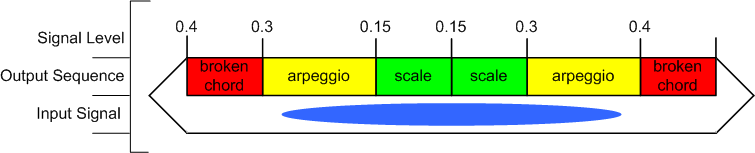
\includegraphics[scale=0.5]{sigmet02}
\caption{Diagram showing how an input signal will result in an output musical sequence by passing a threshold level. In this instance, the signal results in an arpeggio.}
\label{fig:sigmet02}
\end{figure}

\noindent If the signal strength exceeds 0.3 threshold, we get a broken chord returned \textit{(figure \ref{fig:sigmet03})}.

\begin{figure}[ht]
\centering
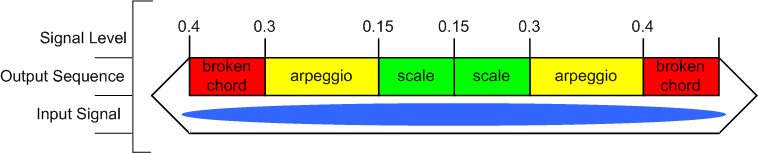
\includegraphics[scale=0.5]{sigmet03}
\caption{Diagram showing how an input signal will result in an output musical sequence by passing a threshold level. In this instance, the signal results in a broken chord.}
\label{fig:sigmet03}
\end{figure}

\section{Programming the Functions for Signal Generation}

The following functions make up the Signal Mapping implementation:
\begin{singlespace}
\begin{formality}
\texttt{prepareAccounts()}: Function to prepare the accounts and return a list of pairs. \\

\texttt{generateSignals( accounts )}: This function generates a list of signals from two accounts. The accounts are expected to be inputted as a list of pairs. \\

\texttt{orderSignals( signals, referenceSignal )}: Function to order the signals from most relevant to least relevant. \\

\texttt{signalProcessorTempo( signal )}: Tempo signal processor. \\

\texttt{getOverallKey( signal )}: Derives a key signature from a signal. \\

\texttt{signalProcessorKey( signal, referenceSignal )}: Key signal processor. Chooses the key based on the signal. As there are 12 notes in an octive (including accidentals), our output value will be between 0 and 11. \\

\texttt{signalCombinator( signals )}: This combines a set of signals into one. \\

\texttt{signalProcessorSequence( signal, referenceSignal, signalPriority )}: Produces a sequence of notes from a signal. \\

\texttt{getStartingNote( signalVariance, cutOff, signalPriority )}: Function to choose a start note within a max and min bounds. \\

\texttt{getStartingOctave( signalPriority )}: Derives a starting octave from a signal. \\

\texttt{signalProcessorScale( signal, signalVariance, signalPriority, referenceSignal )}: Produces a scale from a signal. \\

\texttt{signalProcessorArpeggio( signal, signalVariance, signalPriority, referenceSignal )}: Produces an arpeggio from a signal. \\

\texttt{signalProcessorBrokenChord( signal, signalVariance, signalPriority, referenceSignal )}: Produces a broken chord from a signal. \\

\texttt{createFullScale( octaveTemplate )}: Function to produce a complete scale for 12 octives \\

\texttt{shiftKey( octaveTemplate, keyShift )}: Function to shift the key. \\

\texttt{getKeyMap( octaveTemplate, keyShift )}: Function to produce a map of notes for a given key. \\

\texttt{mapToKey( musicalSequence, keyMap )}: Function to force a note sequence to map its self to a keyMap. \\
\end{formality}
\end{singlespace}

\noindent There is a \texttt{main()}  function which is invoked when the program is first run:

\begin{singlespace}
\begin{formality}

main( argv ): The \texttt{main( argv )} function which is invoked when the program is run. It reads the accounts, and then outputs the music.

\end{formality}
\end{singlespace}

\noindent By looking at the \texttt{main()} function, we can get a good idea of the stages that the program goes through to derive music. The pseudocode for this is given below:

\begin{singlespace}
\begin{formality}
\begin{itemize}
	\item[\textbullet] \texttt{main( argv ):}
	\begin{itemize}
		\item[\textbullet] \texttt{Read in accounts}
		\item[\textbullet] \texttt{Generate signals from accounts}
		\item[\textbullet] \texttt{Generate referenceSignal from signals}
		\item[\textbullet] \texttt{Calculate tempo from referenceSignal}
		\item[\textbullet] \texttt{Calculate key from referenceSignal}
		\item[\textbullet] \texttt{Re-order signals according to how far the deviate from referenceSignal}
		\item[\textbullet] \texttt{Initialise musicalSequences to empty list}
		\item[\textbullet] \texttt{For each signal in signals:}
		\begin{itemize}
			\item[\textbullet] \texttt{Produce a musicalSequence from signal}
			\item[\textbullet] \texttt{Append musicalSequence to musicalSequences}
		\end{itemize}
		\item[\textbullet] \texttt{If parallel approach:}
		\begin{itemize}
			\item[\textbullet] \texttt{derive overallKey from referenceSignal}
			\item[\textbullet] \texttt{for each musicalSequence in musicalSequences:}
			\begin{itemize}
				\item[\textbullet] \texttt{Shift musicalSequence into overallKey}
			\end{itemize}
			\item[\textbullet] \texttt{outputMusic = musicalSequences}
		\end{itemize}
		\item[\textbullet] \texttt{Else if sequential approach:}
		\begin{itemize}
			\item[\textbullet] \texttt{Initialise outputMusic}
			\item[\textbullet] \texttt{for each musicalSequence in musicalSequences:}
			\begin{itemize}
				\item[\textbullet] \texttt{Append musicalSequence to musicalSequences}
			\end{itemize}
		\item[\textbullet] \texttt{Send outputMusic to be played}
		\end{itemize}
	\end{itemize}
\end{itemize}
\end{formality}
\end{singlespace}

\noindent The above algorithm shows that the \texttt{main()} function dervies signals from the attributes. It then derives a reference signal (which is the same as the compound signal described earlier). This reference signal is used to calculate the tempo and overall key signature.

Next, we iterate through each signal and produce a musical sequence. Each musical sequence is appended to a list. We then consider whether we are using the sequential or parallel approach.

If we are using the parallel approach, we iterate through each music sequence and shift them into the overall key. If we are using the sequential approach, we keep each musical sequence in its current key, but we append them to each other so they play in sequence. Finally, we play (or output) the music sequence or sequences.

\section{Summary}

In this chapter we have developed a primary approach towards generating music from accounts. We have seen how we can derive signals from account attribute, and match these to musical sequences.

In the next chapter, we will attempt another approach to music generation by using biological inspiration.